\documentclass[journal,12pt,twocolumn]{IEEEtran}
%
\usepackage{setspace}
\usepackage{gensymb}
\usepackage{siunitx}
\usepackage{tkz-euclide} 
\usepackage{textcomp}
\usepackage{standalone}
\usetikzlibrary{calc}
\newcommand\hmmax{0}
\newcommand\bmmax{0}

%\doublespacing
\singlespacing

%\usepackage{graphicx}
%\usepackage{amssymb}
%\usepackage{relsize}
\usepackage[cmex10]{amsmath}
%\usepackage{amsthm}
%\interdisplaylinepenalty=2500
%\savesymbol{iint}
%\usepackage{txfonts}
%\restoresymbol{TXF}{iint}
%\usepackage{wasysym}
\usepackage{amsthm}
%\usepackage{iithtlc}
\usepackage{mathrsfs}
\usepackage{txfonts}
\usepackage{stfloats}
\usepackage{bm}
\usepackage{cite}
\usepackage{cases}
\usepackage{subfig}
%\usepackage{xtab}
\usepackage{longtable}
\usepackage{multirow}
%\usepackage{algorithm}
%\usepackage{algpseudocode}
\usepackage{enumitem}
\usepackage{mathtools}
\usepackage{steinmetz}
\usepackage{tikz}
\usepackage{circuitikz}
\usepackage{verbatim}
\usepackage{tfrupee}
\usepackage[breaklinks=true]{hyperref}
%\usepackage{stmaryrd}
\usepackage{tkz-euclide} % loads  TikZ and tkz-base
%\usetkzobj{all}
\usetikzlibrary{calc,math}
\usepackage{listings}
    \usepackage{color}                                            %%
    \usepackage{array}                                            %%
    \usepackage{longtable}                                        %%
    \usepackage{calc}                                             %%
    \usepackage{multirow}                                         %%
    \usepackage{hhline}                                           %%
    \usepackage{ifthen}                                           %%
  %optionally (for landscape tables embedded in another document): %%
    \usepackage{lscape}     
\usepackage{multicol}
\usepackage{chngcntr}
\usepackage{amsmath}
\usepackage{cleveref}
\usepackage{amsmath}
%\usepackage{enumerate}

%\usepackage{wasysym}
%\newcounter{MYtempeqncnt}
\DeclareMathOperator*{\Res}{Res}
%\renewcommand{\baselinestretch}{2}
\renewcommand\thesection{\arabic{section}}
\renewcommand\thesubsection{\thesection.\arabic{subsection}}
\renewcommand\thesubsubsection{\thesubsection.\arabic{subsubsection}}

\renewcommand\thesectiondis{\arabic{section}}
\renewcommand\thesubsectiondis{\thesectiondis.\arabic{subsection}}
\renewcommand\thesubsubsectiondis{\thesubsectiondis.\arabic{subsubsection}}

% correct bad hyphenation here
\hyphenation{op-tical net-works semi-conduc-tor}
\def\inputGnumericTable{}                                 %%

\lstset{
%language=C,
frame=single, 
breaklines=true,
columns=fullflexible
}
%\lstset{
%language=tex,
%frame=single, 
%breaklines=true
%}
\usepackage{graphicx}
\usepackage{pgfplots}

\begin{document}


\newtheorem{theorem}{Theorem}[section]
\newtheorem{problem}{Problem}
\newtheorem{proposition}{Proposition}[section]
\newtheorem{lemma}{Lemma}[section]
\newtheorem{corollary}[theorem]{Corollary}
\newtheorem{example}{Example}[section]
\newtheorem{definition}[problem]{Definition}
%\newtheorem{thm}{Theorem}[section] 
%\newtheorem{defn}[thm]{Definition}
%\newtheorem{algorithm}{Algorithm}[section]
%\newtheorem{cor}{Corollary}
\newcommand{\BEQA}{\begin{eqnarray}}
\newcommand{\EEQA}{\end{eqnarray}}
\newcommand{\define}{\stackrel{\triangle}{=}}
\bibliographystyle{IEEEtran}
%\bibliographystyle{ieeetr}
\providecommand{\mbf}{\mathbf}
\providecommand{\abs}[1]{\ensuremath{\left\vert#1\right\vert}}
\providecommand{\norm}[1]{\ensuremath{\left\lVert#1\right\rVert}}
\providecommand{\mean}[1]{\ensuremath{E\left[ #1 \right]}}
\providecommand{\pr}[1]{\ensuremath{\Pr\left(#1\right)}}
\providecommand{\qfunc}[1]{\ensuremath{Q\left(#1\right)}}
\providecommand{\sbrak}[1]{\ensuremath{{}\left[#1\right]}}
\providecommand{\lsbrak}[1]{\ensuremath{{}\left[#1\right.}}
\providecommand{\rsbrak}[1]{\ensuremath{{}\left.#1\right]}}
\providecommand{\brak}[1]{\ensuremath{\left(#1\right)}}
\providecommand{\lbrak}[1]{\ensuremath{\left(#1\right.}}
\providecommand{\rbrak}[1]{\ensuremath{\left.#1\right)}}
\providecommand{\cbrak}[1]{\ensuremath{\left\{#1\right\}}}
\providecommand{\lcbrak}[1]{\ensuremath{\left\{#1\right.}}
\providecommand{\rcbrak}[1]{\ensuremath{\left.#1\right\}}}
\theoremstyle{remark}
\newtheorem{rem}{Remark}
\newcommand{\sgn}{\mathop{\mathrm{sgn}}}
\providecommand{\res}[1]{\Res\displaylimits_{#1}} 
%\providecommand{\norm}[1]{\lVert#1\rVert}
\providecommand{\mtx}[1]{\mathbf{#1}}
\providecommand{\fourier}{\overset{\mathcal{F}}{ \rightleftharpoons}}
%\providecommand{\hilbert}{\overset{\mathcal{H}}{ \rightleftharpoons}}
\providecommand{\system}{\overset{\mathcal{H}}{ \longleftrightarrow}}
	%\newcommand{\solution}[2]{\textbf{Solution:}{#1}}
\newcommand{\solution}{\noindent \textbf{Solution: }}
\newcommand{\cosec}{\,\text{cosec}\,}
\providecommand{\dec}[2]{\ensuremath{\overset{#1}{\underset{#2}{\gtrless}}}}
\newcommand{\myvec}[1]{\ensuremath{\begin{pmatrix}#1\end{pmatrix}}}
\newcommand{\mydet}[1]{\ensuremath{\begin{vmatrix}#1\end{vmatrix}}}
%\numberwithin{equation}{section}
\numberwithin{equation}{subsection}
%\numberwithin{problem}{section}
%\numberwithin{definition}{section}
\makeatletter
\@addtoreset{figure}{problem}
\makeatother
\let\StandardTheFigure\thefigure
\let\vec\mathbf
%\renewcommand{\thefigure}{\theproblem.\arabic{figure}}
\renewcommand{\thefigure}{\theproblem}
%\setlist[enumerate,1]{before=\renewcommand\theequation{\theenumi.\arabic{equation}}
%\counterwithin{equation}{enumi}
%\renewcommand{\theequation}{\arabic{subsection}.\arabic{equation}}
\def\putbox#1#2#3{\makebox[0in][l]{\makebox[#1][l]{}\raisebox{\baselineskip}[0in][0in]{\raisebox{#2}[0in][0in]{#3}}}}
     \def\rightbox#1{\makebox[0in][r]{#1}}
     \def\centbox#1{\makebox[0in]{#1}}
     \def\topbox#1{\raisebox{-\baselineskip}[0in][0in]{#1}}
\vspace{3cm}
\title{Two Classes}
\maketitle
\newpage
%\tableofcontents
\bigskip
\renewcommand{\thefigure}{\theenumi}
\renewcommand{\thetable}{\theenumi}
\begin{abstract}
This document contains theory involved in curve fitting.
\end{abstract}
\section{\textbf{Objective}}
The objective is to use discriminant function to classify.
\section{Generate Dataset}
Create a function of the form
\begin{align}
    y = \vec{w}^{T}\vec{x} + w_{0} \label{eq:1}
\end{align}
This set consists of N samples of input data i.e. x expressed as shown below
\begin{align}
    x = \myvec{x_{1}, x_{2}, .., x_{N}}^{T}
\end{align}
which give the corresponding values of y denoted as
\begin{align}
    y = \myvec{y_{1}, y_{2}, .., y_{N}}^{T}
\end{align}

The corresponding values of y are generated from the Eq \eqref{eq:1}.
The generated input matrix would look like
\begin{align}
    \vec{F}= \myvec{ 1 & x_{0} & x_{0}^2 & \ldots & x_{0}^{N-1} \\
		1 & x_{1} & x_{1}^2 & \ldots & x_{1}^{N-1} \\
		1 & x_{2} & x_{2}^2 & \ldots & x_{2}^{N-1} \\
		\vdots & & \vdots &  & \vdots  \\
		    1 & \ldots & \ldots & \ldots & x_{N}^{N-1} }\label{eq:12}
\end{align}

\section{Linear Discriminant Function (2 Classes)}
The simplest representation of linear discriminant function is
\begin{align}
    y(\vec{x}) = \vec{w}^T\vec{x} + w_{0}
\end{align}
where $w_{0}$ is the bias. The negative of bias is sometimes referred to as threshold.

An input vector $\vec{x}$ is assigned to class $C_{1}$ if $y(\vec{x}) >=0$ and to class $C_{2}$ otherwise.

$y(\vec{x}) = 0$ defines the decision boundary, which corresponds to $(D - 1)$ dimensional hyperplane within the $D$ dimensional input space.

The normal distance from origin to the decision surface is
\begin{align}
    \frac{\vec{w}^T\vec{x}}{\norm{\vec{w}}} = \frac{w_{0}}{\norm{\vec{w}}}
\end{align}

The value of $y(\vec{x})$ gives us the measure of the perpendicular distance $r$ from the point $\vec{x}$ to the decision surface.

Consider an arbitrary point $\vec{x}$ and $\vec{x}_{\perp}$ is its orthogonal projection onto the decision surface
\begin{align}
    \vec{x} = \vec{x}_{\perp} + r \frac{\vec{w}}{\norm{\vec{w}}} \label{eq : a}
\end{align}
we have
\begin{align}
    y(\vec{x}) = \vec{w}^T\vec{x} + w_{0}\label{eq : b}\\
    y(\vec{x}_{\perp}) = \vec{w}^T\vec{x}_{\perp} + w_{0}\label{eq : c}
\end{align}
Using Eq \eqref{eq : a}, Eq \eqref{eq : b} and Eq \eqref{eq : c},
\begin{align}
    r = \frac{y(\vec{x})}{\norm{\vec{w}}}
\end{align}
For a compact notation, we introduce dummy input value $x_{0} = 1$ and then define 
\begin{align}
    \overline{\vec{w}} = \brak{w_{0},\vec{w}}\\
    \overline{\vec{x}} = \brak{x_{0},\vec{x}}
\end{align}
So that,
\begin{align}
    y(\vec{x}) = \overline{\vec{w}}^{T}\overline{\vec{x}}
\end{align}
In order to find a good projection vector, we need to define a measure
of separation between the projections.

Consider there are $N_{1}$ points of class $C_{1}$ and $N_{2}$ points of class $C_{2}$

The mean vector of the two classes are
\begin{align}
      \mu_{1} = \frac{1}{N_{1}} \sum_{\vec{x} \epsilon C_{1}} \vec{x}\\
      \mu_{2} = \frac{1}{N_{2}} \sum_{\vec{x} \epsilon C_{2}} \vec{x}
\end{align}
The mean vector in y feature space is
\begin{align}
    \overline{\mu_{1}} = \frac{1}{N_{1}} \sum_{y \epsilon C_{1}} y = \frac{1}{N_{1}} \sum_{\vec{x} \epsilon C_{1}} \vec{w}^T\vec{x} = \vec{w}^{T}\mu_{1}\label{eq : mean}\\
    \overline{\mu_{2}} = \frac{1}{N_{2}} \sum_{y \epsilon C_{2}} y = \frac{1}{N_{2}} \sum_{\vec{x} \epsilon C_{2}} \vec{w}^T\vec{x} = \vec{w}^{T}\mu_{2}
\end{align}
We could choose the objective function as the distance between the projected means
\begin{align}
    J(\vec{w}) = \abs{\overline{\mu_{1}} - \overline{\mu_{2}}} =\abs{ \vec{w}^{T}\brak{\mu_{1} - \mu_{2}}}
\end{align}
The distance between the projected means is not very good as it doesn't involve standard deviations with in the classes.

For each class we define the scatter, an equivalent of the variance, as
\begin{align}
    \overline{s_{1}}^2 = \sum_{y \epsilon C_{1}} (y - \overline{\mu_{1}})^2\\
    \overline{s_{2}}^2 = \sum_{y \epsilon C_{2}} (y - \overline{\mu_{2}})^2 \label{eq : within_class_scatter}
\end{align}
The quantity $(\overline{s_{1}}^2 + \overline{s_{1}}^2)$, represents the within-class scatter of the projected inputs.

The Fisher linear discriminant is defined as the linear function $\vec{w}^{T}\vec{x}$ that maximizes the objective function
\begin{align}
    J(\vec{w}) = \frac{\abs{\overline{\mu_{1}} - \overline{\mu_{2}}}^2}{\overline{s_{1}}^2 - \overline{s_{2}}^2}
\end{align}
To find the optimum projection $\vec{w}*$, we need to express $J(\vec{w})$ as an explicit function of $\vec{w}$ .

We define a measure of the scatter in multivariate feature space $\vec{x}$ which are co-variance matrices
\begin{align}
    S_{1} = \sum_{x \epsilon C_{1}}\brak{\vec{x} - \mu_{1}}\brak{\vec{x} - \mu_{1}}^{T}\\
    S_{2} = \sum_{x \epsilon C_{2}}\brak{\vec{x} - \mu_{2}}\brak{\vec{x} - \mu_{2}}^{T}\\
    S_{1} + S_{2} = S_{w}
\end{align}
where $S_{w}$ is called the \textbf{within-class} co-variance matrix

The scatter of the projection y can then be expressed as a function of the scatter matrix in
feature space $\vec{x}$
\begin{multline}
    \overline{s_{1}}^2 = \sum_{y \epsilon C_{1}} (y - \overline{\mu_{1}})^2\\
          =\sum_{x \epsilon C_{1}} \brak{\vec{w}^{T}\vec{x} - \vec{w}^{T}\mu_{1}}^2 = \sum_{x \epsilon C_{1}} \vec{w}^{T}\brak{\vec{x} - \mu_{1}}\brak{\vec{x} - \mu_{1}}^{T}\vec{w}\\
          =\vec{w}^{T}S_{1}\vec{w}
\end{multline}
Similarily,
\begin{align}
    \overline{s_{2}}^2 = \vec{w}^{T}S_{2}\vec{w}\\
    \overline{s_{1}}^2 + \overline{s_{2}}^2 = \vec{w}^{T} S_{w} \vec{w}
\end{align}

Similarly, the difference between the projected means can be expressed in terms of the means
in the original feature space

\begin{multline}
    \brak{\overline{\mu_{1}} - \overline{\mu_{2}}}^2 = \brak{\vec{w}^{T}\mu_{1} - \vec{w}^{T}\mu_{2}}^{2}\\
    =\vec{w}^{T}\brak{\mu_{1} - \mu_{2}}\brak{\mu_{1} - \mu_{2}}^{T}\vec{w} = \vec{w}^{T}S_{B}\vec{w}
\end{multline}
where, $S_{B} = \brak{\mu_{1} - \mu_{2}}\brak{\mu_{1} - \mu_{2}}^{T}$ is called \textbf{between-class} covariance matrix.

since $S_{B}$ is the outer product of two vectors,its rank is at most one.

The Expression of the fisher's criterion in terms of $S_{w}$ and $S_{B}$ is
\begin{align}
     J(\vec{w}) = \frac{\vec{w}^{T}S_{B}\vec{w}}{\vec{w}^{T}S_{w}\vec{w}}
\end{align}
To find the maximum of $J(\vec{w})$ we find the derivation and equate it to zero
\begin{multline}
    \frac{d}{d\vec{w}}\brak{J(\vec{w})} = \frac{d}{d\vec{w}}\brak{\frac{\vec{w}^{T}S_{B}\vec{w}}{\vec{w}^{T}S_{w}\vec{w}}} = 0\\
\implies \brak{\vec{w}^{T}S_{w}\vec{w}}\frac{d}{d\vec{w}}\brak{\vec{w}^{T}S_{B}\vec{w}}\\ 
-\brak{\vec{w}^{T}S_{B}\vec{w}}\frac{d}{d\vec{w}}\brak{\vec{w}^{T}S_{w}\vec{w}} = 0\\
 \implies \brak{\vec{w}^{T}S_{w}\vec{w}}2S_{B}\vec{w} - \brak{\vec{w}^{T}S_{B}\vec{w}}2S_{w}\vec{w} = 0
\end{multline}
Divide by $\vec{w}^{T}S_{w}\vec{w}$,
\begin{multline}
    \brak{\frac{\vec{w}^{T}S_{w}\vec{w}}{\vec{w}^{T}S_{w}\vec{w}}}S_{B}\vec{w} - \brak{\frac{\vec{w}^{T}S_{B}\vec{w}}{\vec{w}^{T}S_{w}\vec{w}}}S_{w}\vec{w} = 0\\
    \implies S_{B}\vec{w} - JS_{w}\vec{w} = 0\\
    \implies S_{w}^{-1}S_{B}\vec{w} - J\vec{w} = 0 \label{eq : abc}
\end{multline}
Solving Eq \eqref{eq : abc} gives us, 
\begin{align}
    \vec{w}^{*} = argmax\brak{\frac{\vec{w}^{T}S_{B}\vec{w}}{\vec{w}^{T}S_{w}\vec{w}}} = S_{w}^{-1}\brak{\mu_{1} - \mu_{2}} \label{eq : fisher_linear_discriminant}
\end{align}
Eq \eqref{eq : fisher_linear_discriminant}, is known as the Fisher's Linear Discriminant
\section{Implementation}
We would perform Linear Discriminant Analysis on iris dataset. The Iris flower data set or Fisher's Iris data set is a multivariate data set. 

Based on Fisher's linear discriminant model, this data set became a typical test case for many statistical classification techniques in machine learning.

First, we define the LDA class
\begin{lstlisting}
class LDA:
    def __init__(self):
        pass
 
    def fit(self, X, y):
        pass
\end{lstlisting}
Now, we define a function fit() and firstly find the mean of for each class and store them in mean\_vectors list
\begin{lstlisting}
def fit(self, X, y):
        target_classes = np.unique(y)
        mean_vectors = []
 
        for cls in target_classes:
            mean_vectors.append(np.mean(X[y == cls], axis=0))

\end{lstlisting}
Since we use the 2 classes method,then simply calculate the B matrix as per the Eq \eqref{eq : mean},
\begin{lstlisting}
mu1_mu2 = (mean_vectors[0] - mean_vectors[1]).reshape(1, X.shape[1])
B = np.dot(mu1_mu2.T, mu1_mu2)
\end{lstlisting}
Now, we define an empty array s\_matrix to store the co-variance matrix for each class
\begin{lstlisting}
s_matrix = []
 
for cls, mean in enumerate(mean_vectors):
	Si = np.zeros((X.shape[1], X.shape[1]))
	for row in X[y == cls]:
		t = (row - mean).reshape(1, X.shape[1])
		Si += np.dot(t.T, t)
	s_matrix.append(Si)
\end{lstlisting}
Create the S matrix and loop through the s\_matrix list to append all the values.
\begin{lstlisting}
S = np.zeros((X.shape[1], X.shape[1]))
for s_i in s_matrix:
	S += s_i
\end{lstlisting}
Now, we calculate $S^{-1}$ and $S^{-1}B$. Further we get the eigen values and eigen vectors as follows
\begin{lstlisting}
S_inv = np.linalg.inv(S)
 
S_inv_B = S_inv.dot(B)
 
eig_vals, eig_vecs = np.linalg.eig(S_inv_B)
\end{lstlisting}
Now, we define a function to load the iris dataset for running the experiment.
\begin{lstlisting}
def load_data(cols, load_all=False, head=False):
    iris = sns.load_dataset("iris")
 
    if not load_all:
        if head:
            iris = iris.head(100)
        else:
            iris = iris.tail(100)
 
    le = preprocessing.LabelEncoder()
    y = le.fit_transform(iris["species"])
 
    X = iris.drop(["species"], axis=1)
 
    if len(cols) > 0:
        X = X[cols]
 
    return X.values, y
\end{lstlisting}
Since we need to solve the 2 classes problem, we use only 2 classes from the dataset.
\begin{lstlisting}
cols = ["petal_length", "petal_width"]
X, y = load_data(cols, load_all=False, head=True)
print(X.shape)
\end{lstlisting}
Invoke fit() by passing the X and y, which will return all the eigen vectors.
\begin{lstlisting}
lda = LDA()
W = lda.fit(X, y)
\end{lstlisting}
The following block plots the projected space.
\begin{lstlisting}
colors = ['red', 'green', 'blue']
fig, ax = plt.subplots(figsize=(10, 8))
for point, pred in zip(X, y):
    ax.scatter(point[0], point[1], color=colors[pred], alpha=0.3)
    proj = (np.dot(point, W) * W) / np.dot(W.T, W)
 
    ax.scatter(proj[0], proj[1], color=colors[pred], alpha=0.3)
 
plt.show()
\end{lstlisting}
The plot would look like Fig 
\begin{figure}[!h]
\begin{center}
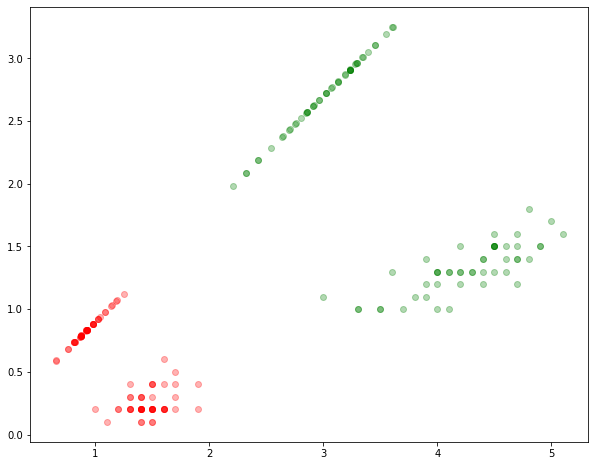
\includegraphics[width=3.4in]{figs/fig1.png}
\end{center}
\caption{}
\label{fig:1}
\end{figure}

In speech dataset, since the input array is of higher dimension, we would use mfccs(Mel Frequency Cepstral Coefficients) as these are proved to be more efficient in feature extraction and classification.

Python code:
\begin{lstlisting}
https://github.com/Hrithikraj2/EE4015_IDP/blob/main/Assignment_8/Assignment_8.ipynb
\end{lstlisting}
\end{document}
